\documentclass[11pt,a4paper]{article}

\usepackage[utf8]{inputenc}
\usepackage[T1]{fontenc}
\usepackage{graphicx}
\usepackage{booktabs}
\usepackage{tabularx}
\usepackage{amsmath,amssymb}
\usepackage{multicol}
\usepackage{needspace}
\usepackage{titlesec}
\usepackage{placeins}
\usepackage{geometry}
\usepackage{caption}
\usepackage{subcaption}
\usepackage{listings}
\usepackage{enumitem}
\usepackage{fancyhdr}
\usepackage{hyperref}
\usepackage{xcolor}
\usepackage{microtype}
\usepackage{float}
\setlength{\emergencystretch}{5em}

\geometry{left=1.5cm,right=1.5cm,top=1.5cm,bottom=1.8cm}

\hypersetup{
  colorlinks=true,
  linkcolor=blue!60!black,
  citecolor=blue!60!black,
  urlcolor=blue!60!black,
}

\captionsetup{font=small,labelfont=bf,skip=2pt}
\numberwithin{table}{section}
\numberwithin{figure}{section}
\setlist{nosep,leftmargin=1.4em}
\setlength{\parskip}{0pt}
\setlength{\parindent}{15pt}
\setlength{\textfloatsep}{4pt plus 1pt minus 1pt}
\setlength{\floatsep}{4pt plus 1pt minus 1pt}
\setlength{\intextsep}{2pt plus 1pt minus 1pt}
\titlespacing*{\section}{0pt}{1.2ex plus 0.2ex minus 0.1ex}{0.6ex plus 0.1ex}
\titlespacing*{\subsection}{0pt}{1.0ex plus 0.2ex minus 0.1ex}{0.5ex plus 0.1ex}
\titlespacing*{\subsubsection}{0pt}{0.8ex plus 0.1ex minus 0.1ex}{0.4ex plus 0.1ex}


\lstset{
  basicstyle=\ttfamily\small,
  breaklines=true,
  frame=single,
  numbers=left,
  numbersep=5pt,
  showstringspaces=false,
}

\pagestyle{plain}

%=====================================================================
%  Project metadata -- EDIT THESE
%=====================================================================
\newcommand{\coursename}{DATA MINING: FUNDAMENTAL}
\newcommand{\projecttitle}{Project report: Seller-Level Vehicle Listings Dataset}
\newcommand{\academicyear}{Academic Year 2026/2027}
\newcommand{\teacherA}{Dino Pedreschi}
\newcommand{\teacherB}{Riccardo Guidotti}
\newcommand{\teacherC}{Alessio Cascione}
\newcommand{\memberA}{Muhammad Iqbal Zain}
\newcommand{\memberB}{Truong Giang Do}
\newcommand{\memberC}{Vladislav Zhelezov}

\begin{document}

%---------------------------------------------------------------------
%  Title page
%---------------------------------------------------------------------
\begin{titlepage}
  \thispagestyle{empty}
  \centering
  \vspace*{1cm}
  
\includegraphics[width=0.28\linewidth]{figures/unipi_logo.png}\\[1.2cm]
  {\Large UNIVERSITY OF PISA}\\[0.3cm]
  {\large DEPARTMENT OF COMPUTER SCIENCE}\\[0.8cm]
  {\large Master programme in Data Science and Business Informatics}\\[2.5cm]
  {\LARGE\bfseries \coursename}\\[0.6cm]
  {\Large \projecttitle}\\[3.5cm]
  \begin{minipage}[t]{0.45\linewidth}
    \raggedright
    Teachers:\\
    \teacherA\\
    \teacherB\\
    \teacherC
  \end{minipage}\hfill
  \begin{minipage}[t]{0.45\linewidth}
    \raggedleft
    Group:\\
    \memberA\\
    \memberB\\
    \memberC
  \end{minipage}\\[3cm]
  \rule{\linewidth}{0.4pt}\\[1cm]
  {\large \academicyear}
\end{titlepage}

%---------------------------------------------------------------------
\pagenumbering{roman}
\tableofcontents
\newpage

%=====================================================================
\pagenumbering{arabic}
\section{Data Understanding and Preparation}
\label{sec:understanding}
\subsection{Data semantics}
\label{sec:semantics}
The Seller-Level Vehicle Listings dataset contains 13,843 records and 33 features. Each record represents a distinct seller (\texttt{sp\_id}) with information on the seller's vehicle listings. A semantic description table is provided below to get a thorough overview of the dataset.
\begin{table}[H]
  \centering
  \caption{Semantic description of the dataset variables. The bold row marks the prediction target.}
  \label{tab:semantics}
  \footnotesize
  \setlength{\tabcolsep}{4.5pt}
  \renewcommand{\arraystretch}{1.05}
  \begin{tabularx}{\textwidth}{l X l l}
    \toprule
    Feature Name & Description & Datatype & Msrmt Scale \\
    \midrule
    \emph{sp\_id} & Unique identifier of the seller/dealer & float64 & Identifier \\
    \emph{n\_listings} & Total number of vehicle listings & int64 & Numerical \\
    \emph{price\_median} & Median advertised price of vehicles & float64 & Numerical \\
    \emph{savings\_amount\_median} & Median advertised savings amount & float64 & Numerical \\
    \emph{daysonmarket\_median} & Median days vehicles remained on market & float64 & Numerical \\
    \emph{mileage\_median} & Median vehicle mileage & float64 & Numerical \\
    \emph{year\_median} & Median vehicle model year & float64 & Numerical \\
    \emph{vehicle\_age\_median} & Median vehicle age at listing time & float64 & Numerical \\
    \emph{owner\_count\_median} & Median number of previous vehicle owners & float64 & Numerical \\
    \emph{horsepower\_median} & Median vehicle horsepower & float64 & Numerical \\
    \emph{engine\_displacement\_median} & Median vehicle engine displacement & float64 & Numerical \\
    \emph{city\_fuel\_economy\_median} & Median city fuel economy & float64 & Numerical \\
    \emph{highway\_fuel\_economy\_median} & Median highway fuel economy & float64 & Numerical \\
    \emph{back\_legroom\_median} & Median rear-seat legroom & float64 & Numerical \\
    \emph{front\_legroom\_median} & Median front-seat legroom & float64 & Numerical \\
    \emph{fuel\_tank\_volume\_median} & Median fuel tank capacity & float64 & Numerical \\
    \emph{height\_median} & Median vehicle height & float64 & Numerical \\
    \emph{length\_median} & Median vehicle length & float64 & Numerical \\
    \emph{width\_median} & Median vehicle width & float64 & Numerical \\
    \emph{pct\_isCab} & Proportion of vehicles previously used as cabs & float64 & Numerical \\
    \emph{pct\_is\_new} & Proportion of vehicles classified as new & float64 & Numerical \\
    \emph{pct\_salvage} & Proportion of vehicles with salvage status & float64 & Numerical \\
    \emph{pct\_theft\_title} & Proportion of vehicles with theft titles & float64 & Numerical \\
    \emph{n\_listing\_days} & Distinct calendar days with observed listings & int64 & Numerical \\
    \emph{listing\_span\_days} & Span in days between earliest and latest listing & int64 & Numerical \\
    \emph{dominant\_body\_type} & Most frequent vehicle body type & str & Categorical \\
    \emph{dominant\_fuel\_type} & Most frequent fuel type & str & Categorical \\
    \emph{dominant\_transmission} & Most frequent transmission type & str & Categorical \\
    \emph{dominant\_wheel\_system} & Most frequent drivetrain configuration & str & Categorical \\
    \emph{dominant\_listing\_color} & Most frequent exterior color & str & Categorical \\
    \emph{franchise\_status} & Franchise status (franchise, independent, etc.) & str & Categorical \\
    \emph{new\_used\_profile} & Inventory composition (new\_only, used\_only, etc.) & str & Categorical \\
    \textbf{\emph{seller\_rating\_class}} & \textbf{Discretized target rating (low, medium, high)} & \textbf{str} & \textbf{Ordinal} \\
    \bottomrule
  \end{tabularx}
\end{table}

\subsection{Distribution of variables and statistics}
\label{sec:distribution}
\subsubsection{Summary of statistics}
\label{sec:summary-stats}
Table~\ref{tab:stats} provides notable descriptions of the primary statistics for each numerical feature. First, the feature magnitudes vary across four orders of scale, from bounded proportions (\texttt{pct\_*} $\in [0,1]$) and cabin dimensions (\texttt{height\_median} mean 65.15 in) to \texttt{price\_median} (up to \$236,438) and \texttt{mileage\_median} (up to 238,541 mi). Therefore, the data should be standardised before fitting distance-based models.

Secondly, volume, pricing, and risk-history features exhibit severe right-skewness. The most extreme are \texttt{pct\_theft\_title} (14.11), \texttt{pct\_salvage} (10.34), \texttt{daysonmarket\_median} (8.75) and \texttt{n\_listings} (5.25). Conversely, \texttt{year\_median} ($-2.25$) and \texttt{back\_legroom\_median} ($-3.53$) are left-skewed.

Finally, \texttt{engine\_displacement\_median} lacks 3,393 records (24.51\%), and sparse risk indicators (\texttt{pct\_theft\_title}, \texttt{pct\_salvage}) yield $\mathrm{IQR}=0$ due to being heavily zero-inflated.

\begin{table}[H]
  \centering
  \caption{Summary statistics for the 24 numerical variables (identifier excluded).}
  \label{tab:stats}
  \footnotesize
  \setlength{\tabcolsep}{3pt}
  \renewcommand{\arraystretch}{0.98}
  \resizebox{\textwidth}{!}{%
  \begin{tabular}{lrrrrrrrrrrrr}
    \toprule
    Variable & Count & Mean & Std & Min & 25\% & 50\% & 75\% & Max & Missing & Skew & Kurtosis & IQR \\
    \midrule
n\_listings & 13843.0 & 118.10 & 137.06 & 5.00 & 25.00 & 70.00 & 168.00 & 4959.00 & 0 & \textbf{5.25} & 120.32 & 143.00 \\
    price\_median & 13843.0 & 23106.14 & 14365.07 & 1699.00 & 12495.00 & 22385.00 & 29888.00 & 236438.00 & 0 & \textbf{3.45} & 34.14 & 17393.00 \\
    savings\_amount\_median & 13843.0 & 446.21 & 519.46 & 0.00 & 0.00 & 358.00 & 734.00 & 9333.00 & 0 & 2.40 & 18.30 & 734.00 \\
    daysonmarket\_median & 13843.0 & 49.15 & 56.06 & 0.00 & 26.00 & 36.00 & 51.00 & 1987.00 & 0 & \textbf{8.75} & 168.60 & 25.00 \\
    mileage\_median & 13842.0 & 51463.27 & 51845.46 & 0.00 & 25.00 & 33596.50 & 96915.75 & 238541.00 & 1 & 0.68 & -0.77 & 96890.75 \\
    year\_median & 13843.0 & 2015.95 & 4.72 & 1960.00 & 2013.00 & 2017.00 & 2020.00 & 2021.00 & 0 & -2.25 & 14.09 & 7.00 \\
    vehicle\_age\_median & 13842.0 & 4.08 & 4.63 & 0.00 & 0.00 & 3.00 & 7.00 & 60.00 & 1 & 2.32 & 14.98 & 7.00 \\
    owner\_count\_median & 13804.0 & 1.43 & 0.62 & 1.00 & 1.00 & 1.00 & 2.00 & 6.00 & 39 & 1.30 & 1.35 & 1.00 \\
    horsepower\_median & 13837.0 & 240.90 & 56.99 & 78.00 & 188.00 & 243.00 & 283.00 & 630.00 & 6 & 0.85 & 2.05 & 95.00 \\
    engine\_displacement\_median & 10450.0 & 2925.08 & 808.08 & 1200.00 & 2400.00 & 2500.00 & 3500.00 & 6800.00 & \textbf{3393} & 1.29 & 2.77 & 1100.00 \\
    city\_fuel\_economy\_median & 13827.0 & 20.65 & 3.96 & 10.00 & 18.00 & 20.00 & 22.00 & 126.00 & 16 & \textbf{8.10} & 185.87 & 4.00 \\
    highway\_fuel\_economy\_median & 13827.0 & 27.88 & 3.98 & 15.00 & 25.00 & 27.50 & 30.00 & 105.00 & 16 & \textbf{3.88} & 66.79 & 5.00 \\
    back\_legroom\_median & 13824.0 & 37.71 & 1.57 & 0.00 & 36.80 & 37.80 & 38.60 & 47.50 & 19 & \textbf{-3.53} & 77.81 & 1.80 \\
    front\_legroom\_median & 13836.0 & 41.89 & 0.77 & 36.60 & 41.30 & 41.80 & 42.20 & 67.00 & 7 & \textbf{3.49} & 88.62 & 0.90 \\
    fuel\_tank\_volume\_median & 13836.0 & 18.35 & 2.93 & 7.15 & 16.40 & 18.25 & 19.20 & 52.00 & 7 & 1.83 & 7.33 & 2.80 \\
    height\_median & 13837.0 & 65.15 & 4.95 & 46.85 & 61.60 & 66.00 & 68.00 & 107.50 & 6 & 0.18 & 0.91 & 6.40 \\
    length\_median & 13837.0 & 191.10 & 10.25 & 151.00 & 184.60 & 189.80 & 192.70 & 282.30 & 6 & 2.18 & 7.59 & 8.10 \\
    width\_median & 13837.0 & 77.02 & 4.97 & 65.70 & 72.90 & 75.55 & 80.00 & 105.90 & 6 & 1.06 & 1.56 & 7.10 \\
    pct\_isCab & 13816.0 & 0.16 & 0.16 & 0.00 & 0.05 & 0.12 & 0.21 & 1.00 & 27 & 2.04 & 5.91 & 0.17 \\
    pct\_is\_new & 13843.0 & 0.27 & 0.32 & 0.00 & 0.00 & 0.00 & 0.59 & 1.00 & 0 & 0.55 & -1.38 & 0.59 \\
    pct\_salvage & 13816.0 & 0.01 & 0.06 & 0.00 & 0.00 & 0.00 & 0.00 & 1.00 & 27 & \textbf{10.34} & 119.82 & \textbf{0.00} \\
    pct\_theft\_title & 13816.0 & 0.00 & 0.02 & 0.00 & 0.00 & 0.00 & 0.00 & 0.76 & 27 & \textbf{14.11} & 427.34 & \textbf{0.00} \\
    n\_listing\_days & 13843.0 & 46.32 & 33.72 & 1.00 & 18.00 & 39.00 & 68.00 & 272.00 & 0 & 0.98 & 0.95 & 50.00 \\
    listing\_span\_days & 13843.0 & 405.59 & 282.37 & 0.00 & 223.00 & 362.00 & 508.00 & 3553.00 & 0 & 2.15 & 9.00 & 285.00 \\
    \bottomrule
  \end{tabular}}
  \par\vspace{2pt}
  {\footnotesize Bold values mark severe skewness ($|\mathrm{Skew}| \ge 3$), substantial missingness ($\ge 1\%$), and zero IQR.}
\end{table}

\subsubsection{Distribution via histograms}
\label{sec:histograms}


Figure~\ref{fig:hist} illustrates the distributions of core attributes covering seller scale, pricing, turnover, and inventory age. Operational scale (\texttt{n\_listings}), pricing (\texttt{price\_median}), and turnover time (\texttt{daysonmarket\_median}) show heavily right-skewed distributions. The majority of sellers list fewer than 500 vehicles and clear inventory within 200 days, whereas the right tail extends to 4,959 listings and 1,987 days.

In addition, the inventory distribution also shows a clear separation between two distinct dealership models: used-car dealers (\texttt{pct\_is\_new} $=0$, high mileage) and new-car dealers (\texttt{pct\_is\_new} $>0$, near-zero mileage). In contrast, \texttt{year\_median} is strongly left-skewed, concentrating mainly in 2013--2020. Besides, among the remaining attributes, \texttt{owner\_count\_median} concentrates mostly at one or two previous owners, while vehicle specifications (\texttt{height\_median}, \texttt{length\_median}, \texttt{front\_legroom\_median}, \texttt{fuel\_tank\_volume\_median}) form high-kurtosis peaks around standard passenger-vehicle dimensions.

\begin{figure}[H]
  \centering
  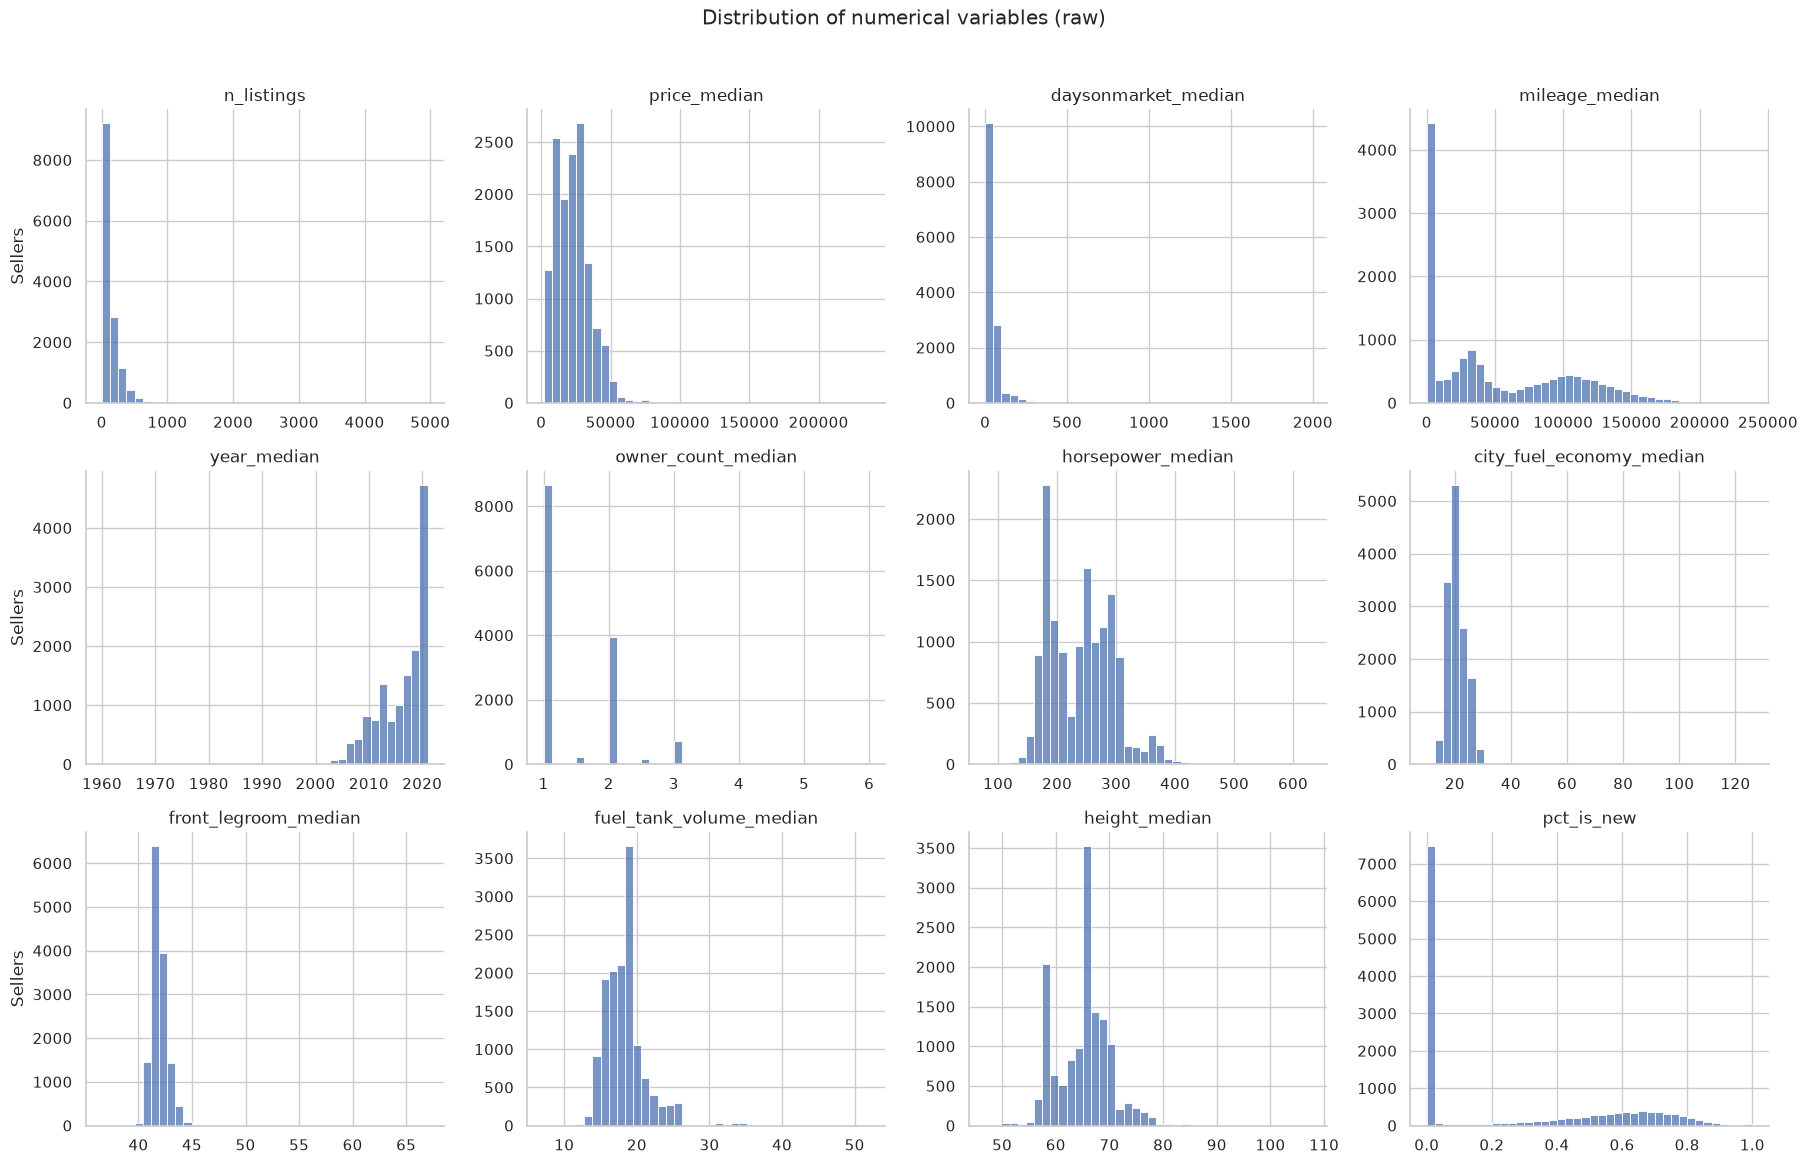
\includegraphics[width=0.9\linewidth]{figures/docx/fig_1_1_histograms.png}
  \caption{Histograms of the selected numerical variables.}
  \label{fig:hist}
\end{figure}

\subsubsection{Distribution of categorical features}
\label{sec:categorical}
\begin{figure}[H]
  \centering
  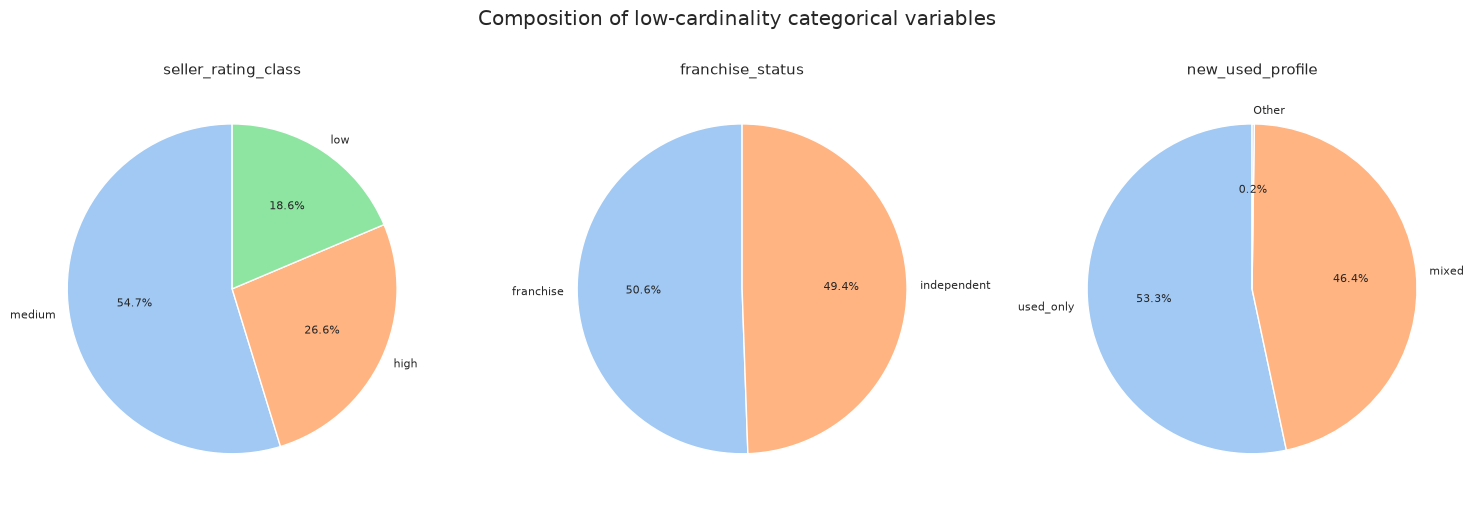
\includegraphics[width=0.80\linewidth]{figures/docx/fig_1_2_pie.png}
  \caption{Composition of the low-cardinality categorical variables.}
  \label{fig:pie}
\end{figure}

The pie charts (Figure~\ref{fig:pie}) show that the target \texttt{seller\_rating\_class} is moderately imbalanced, led by \textit{medium} (54.7\%), followed by \textit{high} (26.6\%) and \textit{low} (18.6\%). In contrast, \texttt{franchise\_status} and \texttt{new\_used\_profile} are evenly split between their values.

\begin{figure}[H]
  \centering
  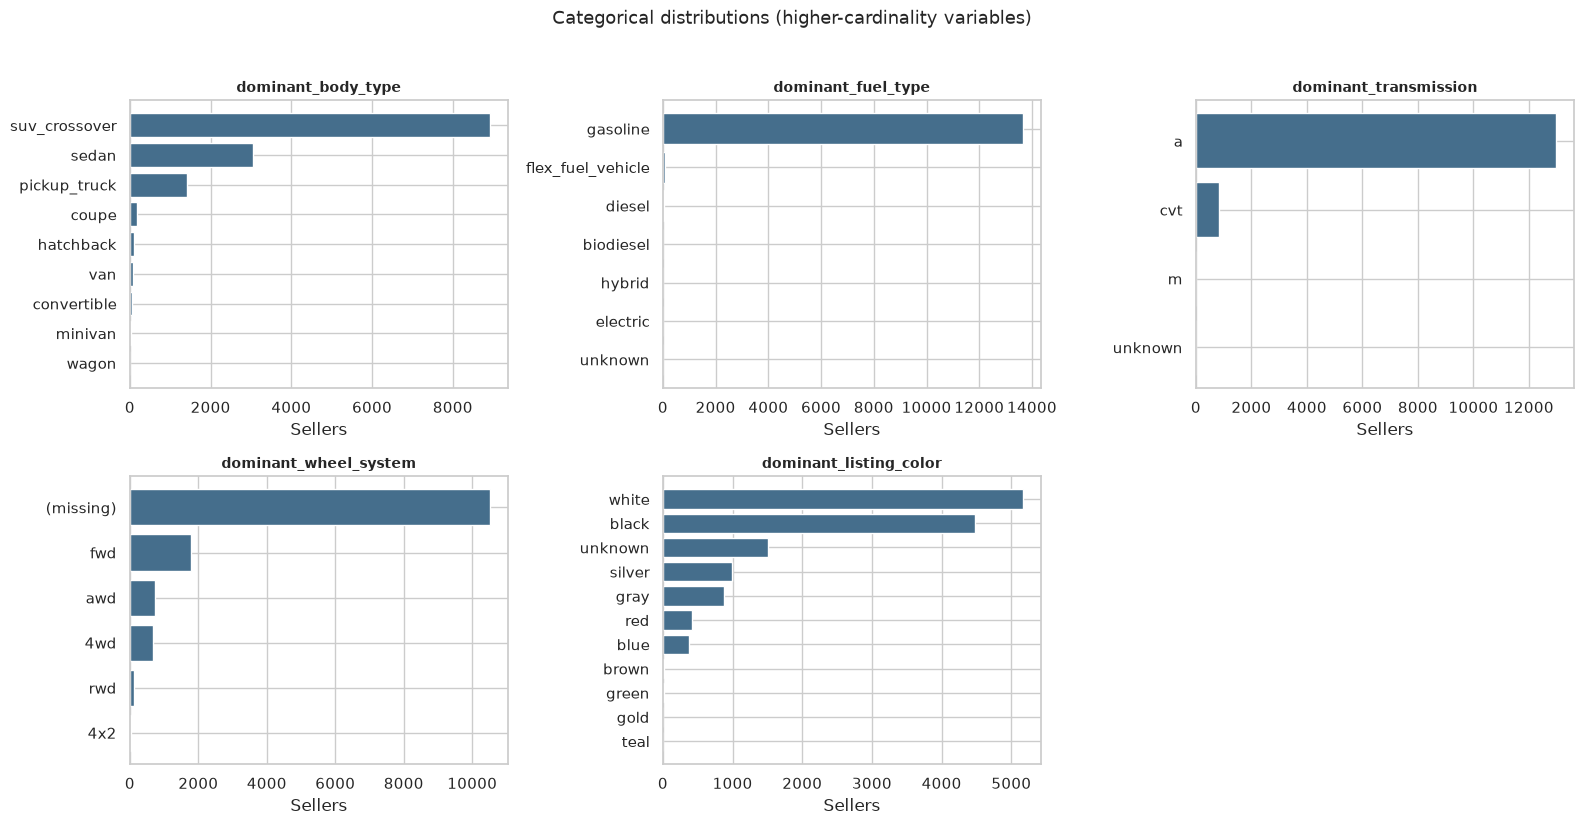
\includegraphics[width=0.85\linewidth]{figures/docx/fig_1_3_bar.png}
  \caption{Distributions of the higher-cardinality categorical variables.}
  \label{fig:bar}
\end{figure}

Among the higher-cardinality features, the bar charts (Figure~\ref{fig:bar}) illustrate that automatic (\texttt{a}) dominates the \texttt{dominant\_transmission} category, while \texttt{dominant\_fuel\_type} is concentrated in \textit{gasoline}. In addition, \texttt{dominant\_listing\_color} is led by neutral colours (white, black, silver, grey), alongside a substantial \textit{unknown} group (10.91\%), while \texttt{dominant\_wheel\_system} is predominantly missing (75.98\%). Lastly, SUVs cover a large proportion (61.1\%) of \texttt{dominant\_body\_type}, followed by sedans (21.8\%) and pickup trucks (12.1\%), leaving all other body types below 5\% in total.

\subsection{Assessment of data quality}
\label{sec:quality}
Our syntactic and semantic audit verified that there are no duplicated rows, specifically among the sellers' identifiers (\texttt{sp\_id}). Secondly, there are no negative values in any numerical attribute. Thirdly, all percentage attributes (\texttt{pct\_isCab}, \texttt{pct\_is\_new}, \texttt{pct\_salvage}, \texttt{pct\_theft\_title}) are correctly bounded within the closed interval $[0,1]$, and advertised discounts never exceed the original prices (\texttt{savings\_amount\_median} $<$ \texttt{price\_median}). Moreover, temporal consistency holds across all records (\texttt{n\_listing\_days} $\leq$ \texttt{n\_listings} and \texttt{n\_listing\_days} $\leq$ \texttt{listing\_span\_days} $+1$).

\begin{sloppypar}
In addition, count and calendar-year medians (\texttt{year\_median}, \texttt{owner\_count\_median}, \texttt{daysonmarket\_median}) contain fractional \texttt{.5} values, which are valid because sellers with an even number of vehicle listings produce them.
\end{sloppypar}

We only made a simple change to the column \texttt{sp\_id}, originally stored as \texttt{float64}, converting it to string.

\subsubsection{Missing value handling}
\label{sec:missing}
There are 20 attributes containing missing values: 17 with explicit \texttt{NaN} values and 3 with implicit \textit{unknown} values (see Table~\ref{tab:missing} and Figure~\ref{fig:missing}).

\begin{table}[H]
  \centering
  \caption{Summary of explicit (\texttt{NaN}) and implicit (\textit{unknown}) missing values. Bold values mark attributes with more than 1\% missing.}
  \label{tab:missing}
  \footnotesize
  \renewcommand{\arraystretch}{1.0}
  \begin{tabularx}{\textwidth}{>{\raggedright\arraybackslash}X r r l}
    \toprule
    Variable & Missing & Missing (\%) & Type \\
    \midrule
    \texttt{dominant\_wheel\_system} & \textbf{10,518} & \textbf{75.98\%} & NaN \\
    \texttt{engine\_displacement\_median} & \textbf{3,393} & \textbf{24.51\%} & NaN \\
    \texttt{dominant\_listing\_color} & \textbf{1,510} & \textbf{10.91\%} & \textit{unknown} \\
    \texttt{dominant\_fuel\_type}, \texttt{dominant\_transmission} & 1--6 & 0.01--0.04\% & \textit{unknown} \\
    \texttt{vehicle\_age\_median} & 1 & 0.01\% & NaN \\
    14 minor numerical attributes\textsuperscript{*} & 1--39 & 0.01--0.28\% & NaN \\
    \bottomrule
  \end{tabularx}
  \par\vspace{2pt}
  {\footnotesize \textsuperscript{*}\texttt{owner\_count\_median}, \texttt{pct\_isCab}, \texttt{pct\_salvage}, \texttt{pct\_theft\_title}, the physical dimensions, legrooms, fuel-economy attributes, \texttt{horsepower\_median}, and \texttt{mileage\_median}.}
\end{table}

\begin{figure}[H]
  \centering
  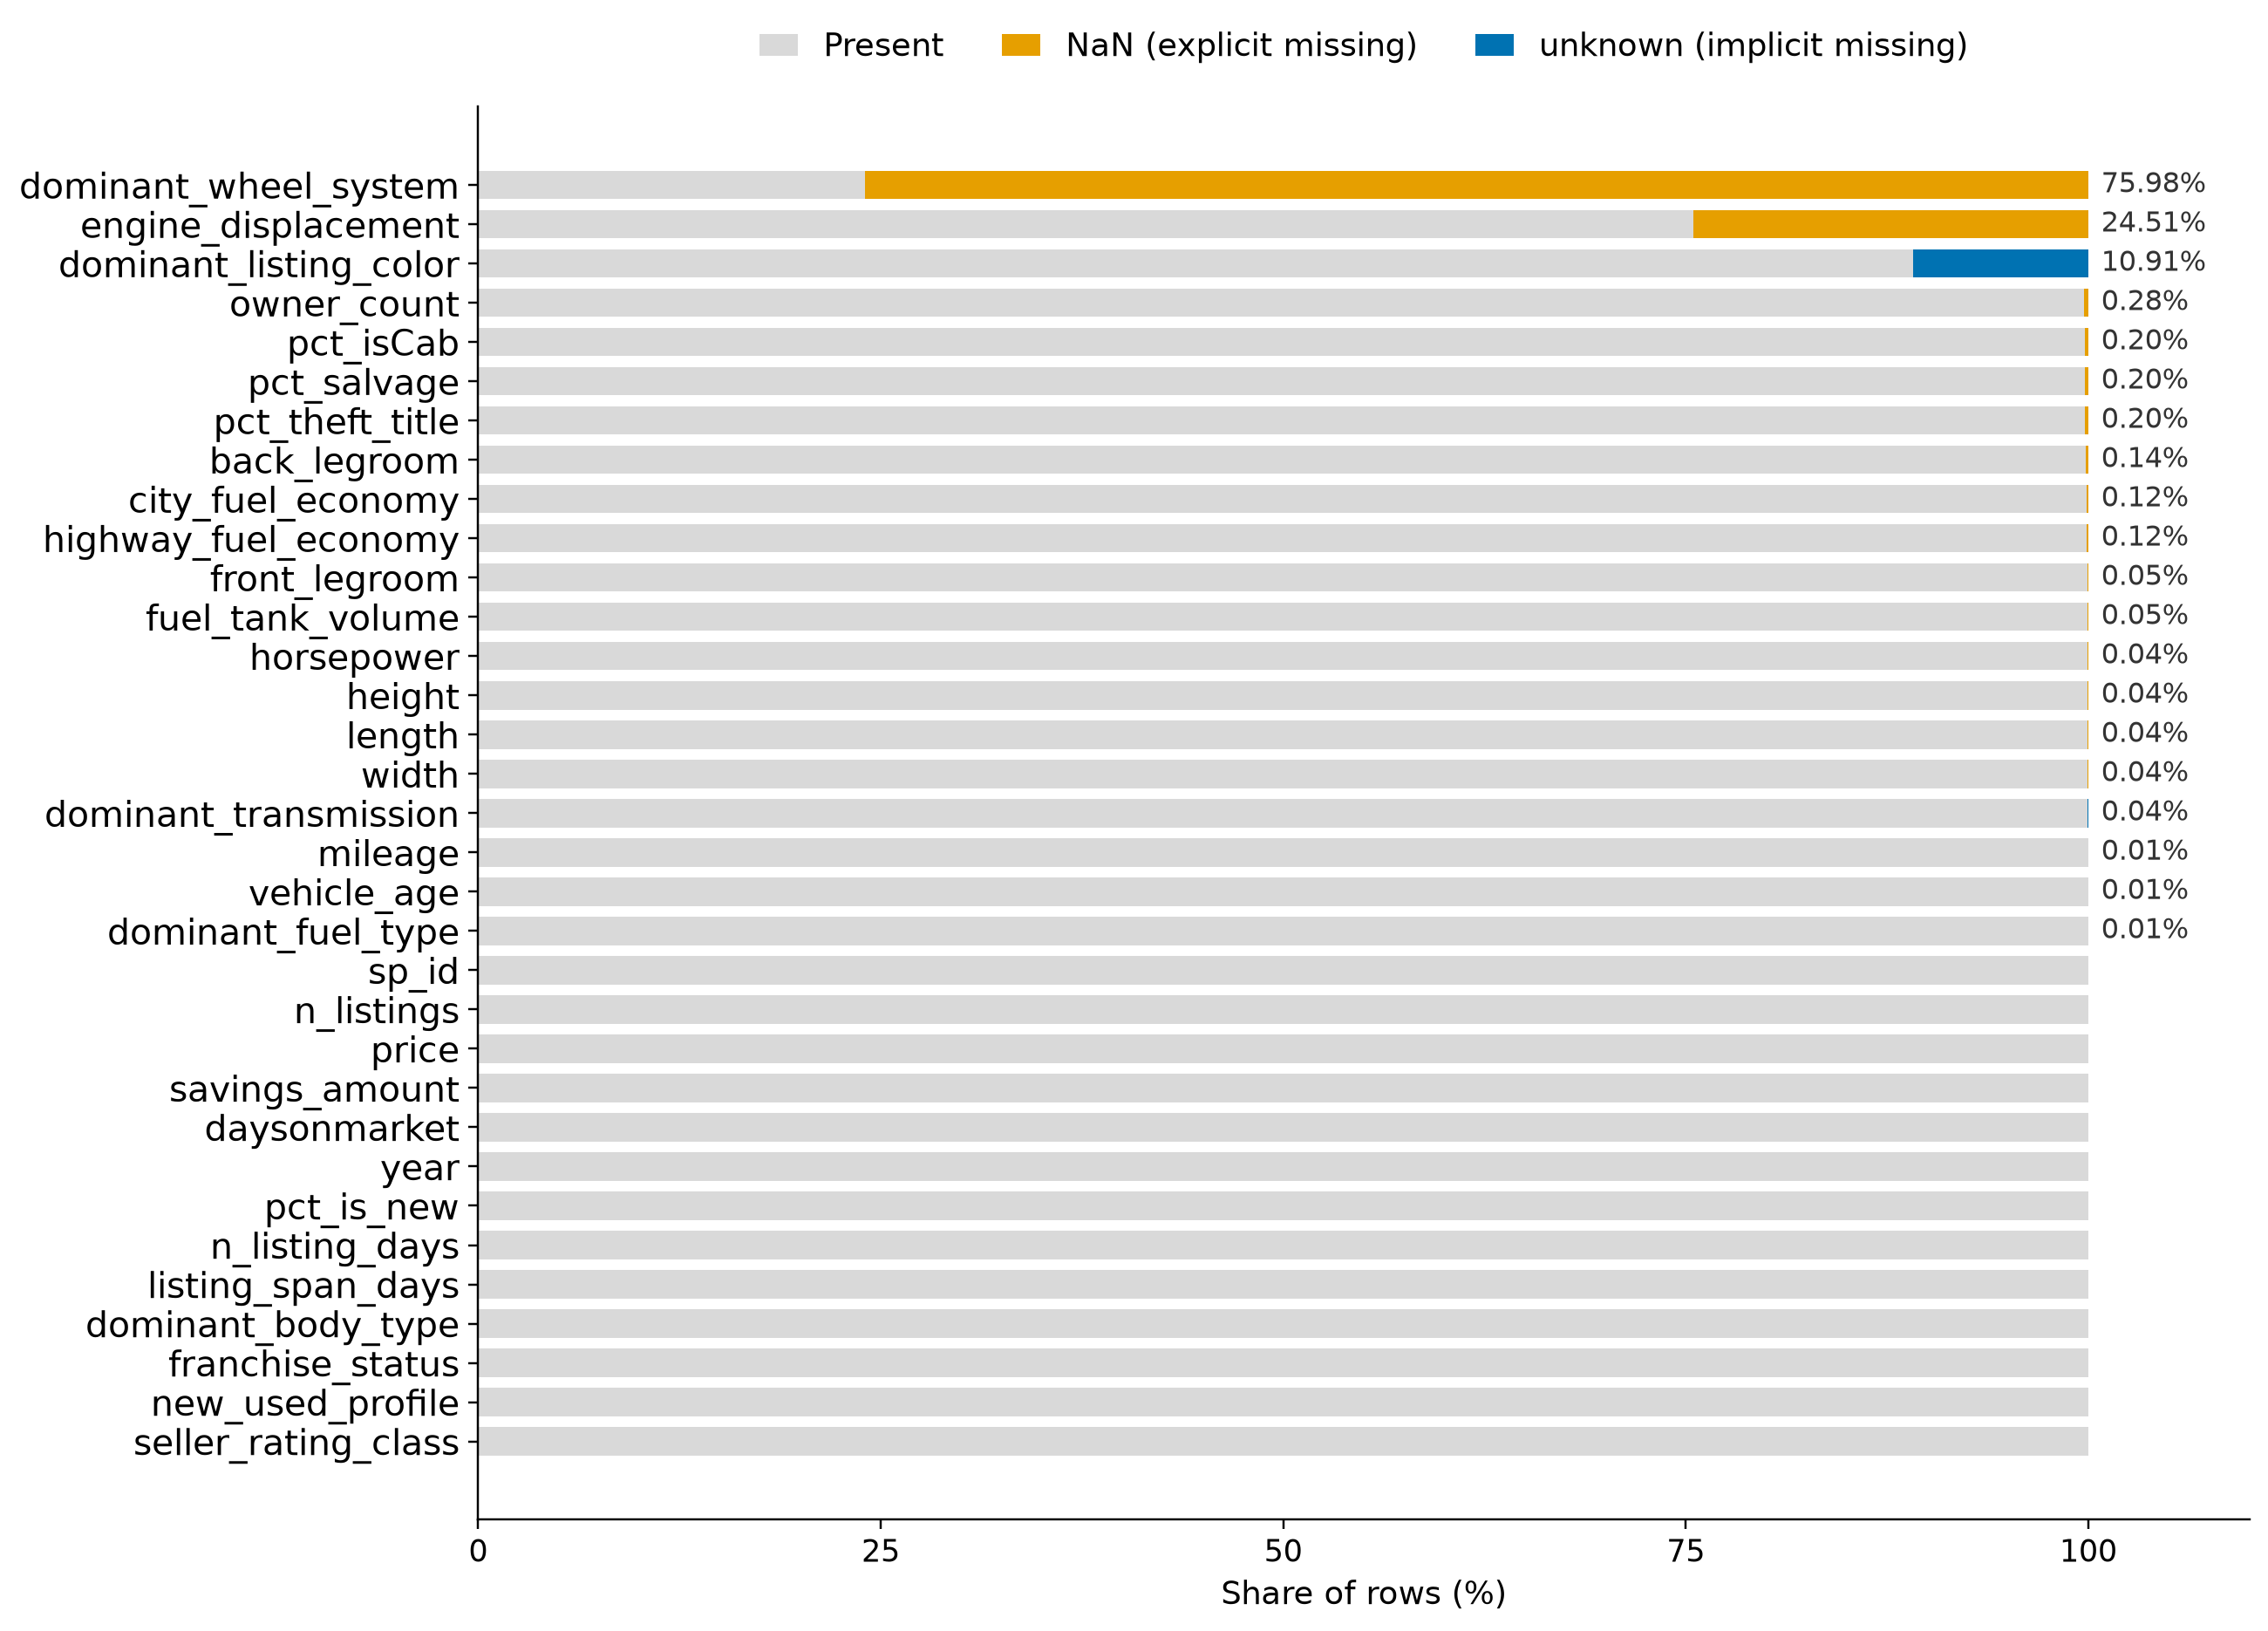
\includegraphics[width=0.85\linewidth]{figures/docx/fig_1_4_missing_barchart.png}
  \caption{Missing-value composition per attribute (sorted by total missing share): explicit \texttt{NaN} and implicit \texttt{unknown} values.}
  \label{fig:missing}
\end{figure}

We applied tailored strategies to handle missing values in each attribute as follows:
\begin{multicols}{2}
\raggedright
\begin{itemize}[leftmargin=*]
  \item \texttt{dominant\_wheel\_system}: dropped due to a high percentage of missing values (75.98\%).
  \item \texttt{engine\_displacement\_median}: missing values (24.51\%) are filled using the median grouped by \texttt{dominant\_body\_type} and \texttt{horsepower\_median} quintiles, which ensures that the engine size reflects both the vehicle's body type and power.
  \item \texttt{dominant\_listing\_color}: implicit \textit{unknown} values (10.91\%) are kept as a separate category, preventing mode substitution from overly skewing the prevalence of the \textit{white} label.
  \item \texttt{dominant\_fuel\_type} and \texttt{dominant\_transmission}: missing values under the implicit \textit{unknown} labels (1 and 6 instances) are converted to the group mode calculated across each \texttt{dominant\_body\_type}.
  \item \texttt{vehicle\_age\_median}: the single missing entry (0.01\%) was computed using the formula $2020 - \texttt{year\_median}$.
  \item The remaining 14 numerical attributes: minor missing values ($<0.30\%$ each) are imputed using the group median calculated across each \texttt{dominant\_body\_type}, preserving expected characteristics across body types.
\end{itemize}
\end{multicols}

\subsubsection{Outlier and noise detection}
\label{sec:outliers}
Inspection of the feature distributions (Figure~\ref{fig:box}) distinguishes true measurement noise from valid domain outliers:

\textbf{True semantic noise.} We identified 3 instances with \texttt{back\_legroom\_median} $=0$ although their \texttt{dominant\_body\_type} is \texttt{suv\_crossover} or \texttt{sedan}. Since this is physically impossible, the values were converted to the group median by body type, as in Section~\ref{sec:missing}.

\textbf{Valid domain outliers.} The \texttt{pct\_salvage} and \texttt{pct\_theft\_title} columns, which recorded 90.83\% and 84.56\% zeros, yield $\mathrm{IQR}=0$. These values represent valid second-hand or salvage dealerships rather than data errors, so we retained all records. Secondly, we examine extreme values across all attributes:
\begin{itemize}[leftmargin=*]
  \item \texttt{n\_listings} (up to 4,959) is verified as a mega-dealership.
  \item \texttt{price\_median} (up to \$236,438), \texttt{horsepower\_median} (up to 630 HP) and \texttt{vehicle\_age\_median} (up to 60 years) are luxury, sport or classic-car dealers.
  \item \texttt{city\_fuel\_economy\_median} (up to 126 MPG) represents electric-car dealers.
  \item \texttt{daysonmarket\_median} (up to 1,987 days) reflects real market heterogeneity, as some dealers have slow-moving inventory.
\end{itemize}

Therefore, all records from these valid sellers were kept to retain niche market segments. In the end, 13,843 records were retained in the cleaned dataset.

\begin{figure}[H]
  \centering
  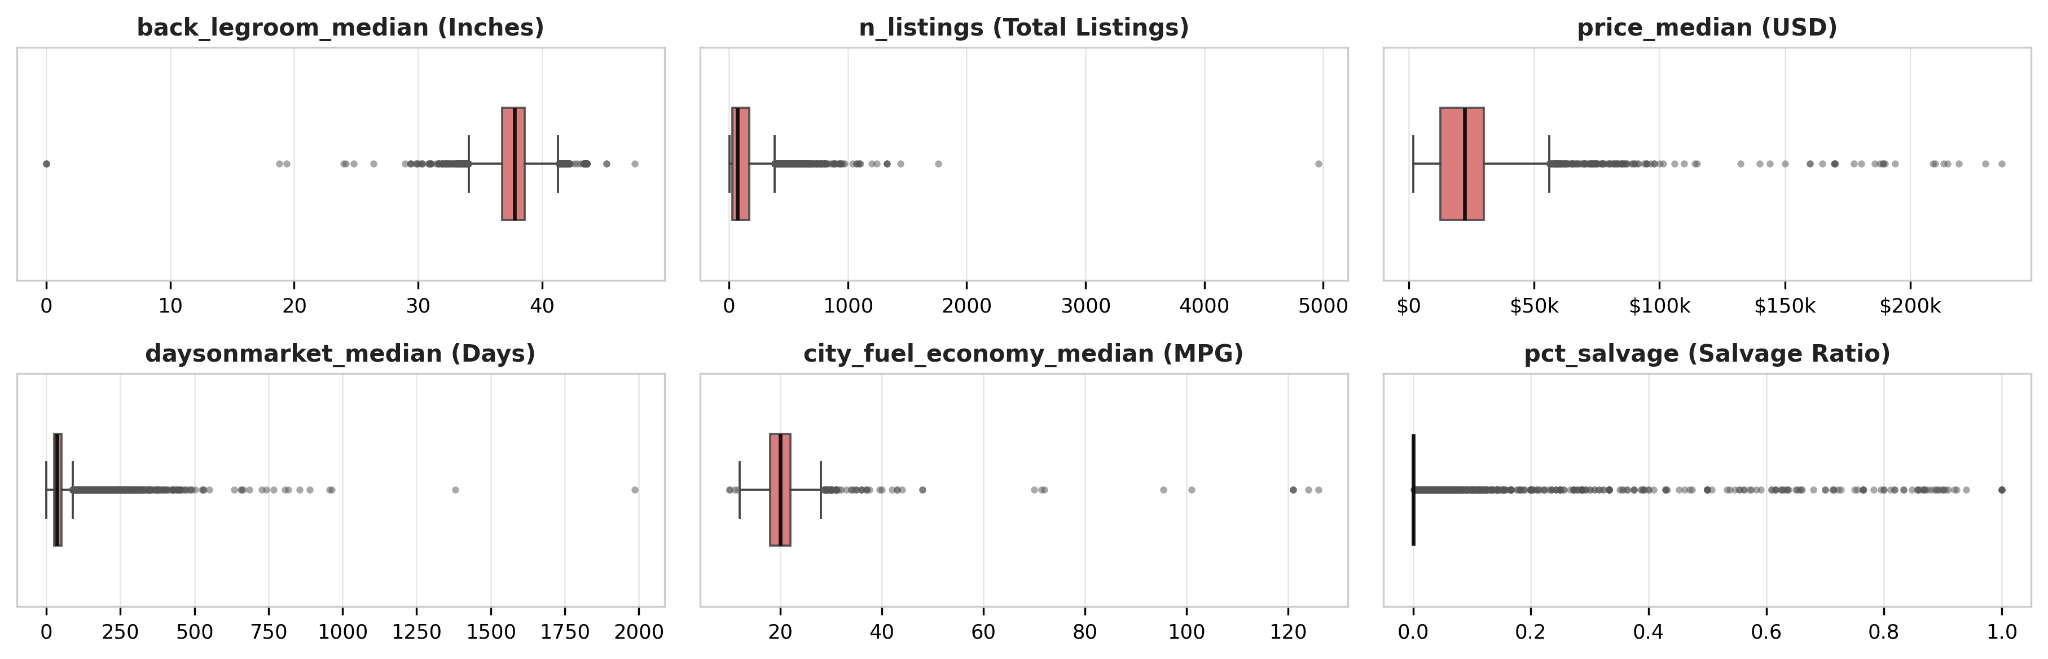
\includegraphics[width=0.9\linewidth]{figures/docx/fig_1_5_boxplots.png}
  \caption{Boxplots of selected numerical attributes for outlier detection.}
  \label{fig:box}
\end{figure}

\subsubsection{Variables transformation}
\label{sec:transform}
To address the heavy right-skewness across the numerical attributes in the dataset, we applied a logarithmic transformation, $\log(1+x)$, to the heavily right-skewed continuous features: \texttt{price\_median}, \texttt{n\_listings}, \texttt{daysonmarket\_median}, \texttt{savings\_amount\_median}, \texttt{vehicle\_age\_median}, \texttt{city\_fuel\_economy\_median}, \texttt{highway\_fuel\_economy\_median}, \texttt{engine\_displacement\_median} and \texttt{fuel\_tank\_volume\_median}. This compresses extreme right tails and restores near-symmetric distributions without undefined values at zero. We then performed feature scaling to ensure uniformity. We generated two standardised representations: Z-score standardisation to mitigate outlier leverage in distance-based algorithms, and Min-Max scaling for bounded metrics.

\needspace{6\baselineskip}
\subsubsection{Pairwise correlations and variable elimination}
\label{sec:correlations}
Inter-feature dependencies were evaluated across the numerical attributes using the pairwise scatter-plot matrix (Figure~\ref{fig:pairwise}) and Spearman's correlation matrix (Figure~\ref{fig:corr}). We selected the Spearman method over Pearson because Figure~\ref{fig:pairwise} reveals strong non-linear monotonic patterns: specifically, \texttt{price\_median} drops sharply as \texttt{mileage\_median} and \texttt{vehicle\_age\_median} increase before flattening out, forming an L-shaped curve alongside the heavy right-tail outliers.

The correlation matrix also shows some important findings. Firstly, regarding highly correlated pairs, we retained both \texttt{mileage\_median} and \texttt{vehicle\_age\_median} (0.93) as well as \texttt{n\_listings} and \texttt{n\_listing\_days} (0.96) in the master dataset, because their relative ratios capture annual vehicle usage and active posting intensity. Secondly, within the technical specifications, \texttt{engine\_displacement\_median} correlates positively with \texttt{fuel\_tank\_volume\_median} (0.79) and \texttt{horsepower\_median} (0.77), but negatively with \texttt{city\_fuel\_economy\_median} ($-0.76$), reflecting the trade-off between engine capacity and fuel efficiency.

Finally, we removed \texttt{year\_median} ($-0.98$ with \texttt{vehicle\_age\_median}, since the latter equals $2020 - \texttt{year\_median}$) and \texttt{highway\_fuel\_economy\_median} (0.94 with \texttt{city\_fuel\_economy\_median}, as they describe identical fuel efficiency), resulting in a final prepared dataset of 13,843 rows and 29 attributes.

\begin{figure}[t]
\begin{minipage}[t]{0.48\linewidth}
  \centering
  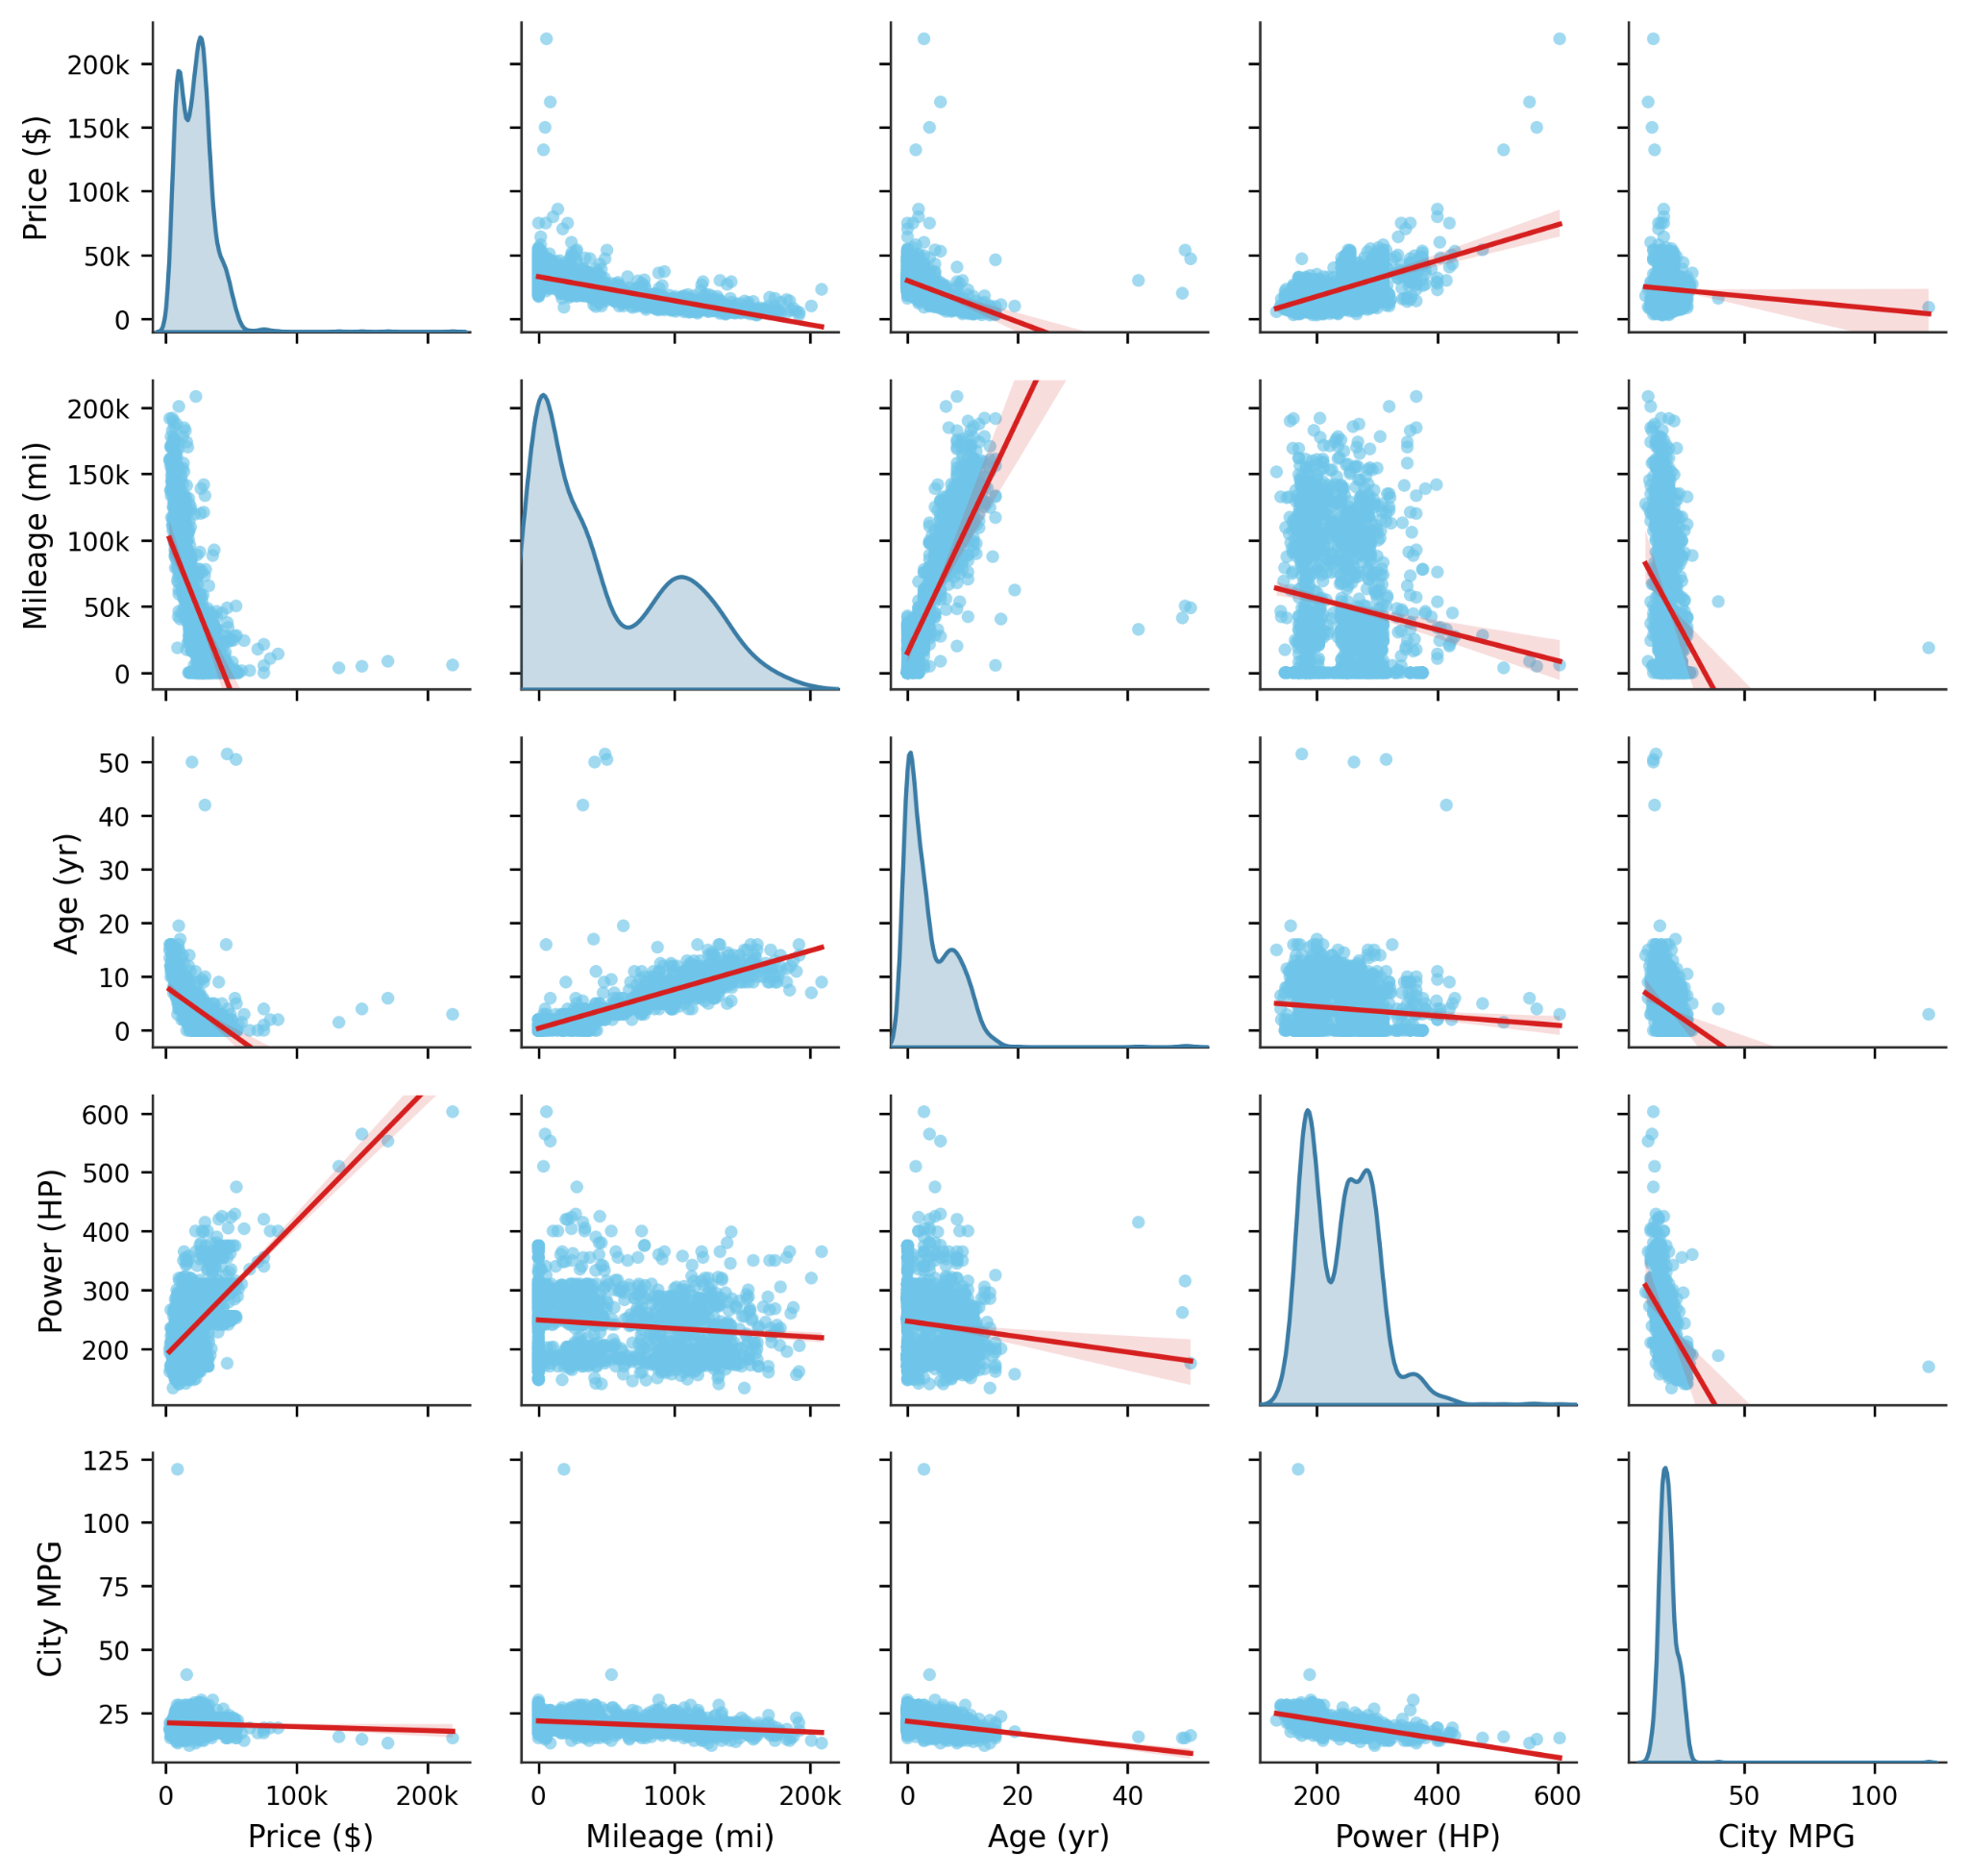
\includegraphics[width=\linewidth]{figures/docx/fig_1_6_pairwise.png}
  \captionof{figure}{Pairwise scatter-plot matrix of the key numerical attributes.}
  \label{fig:pairwise}
\end{minipage}\hfill
\begin{minipage}[t]{0.48\linewidth}
  \centering
  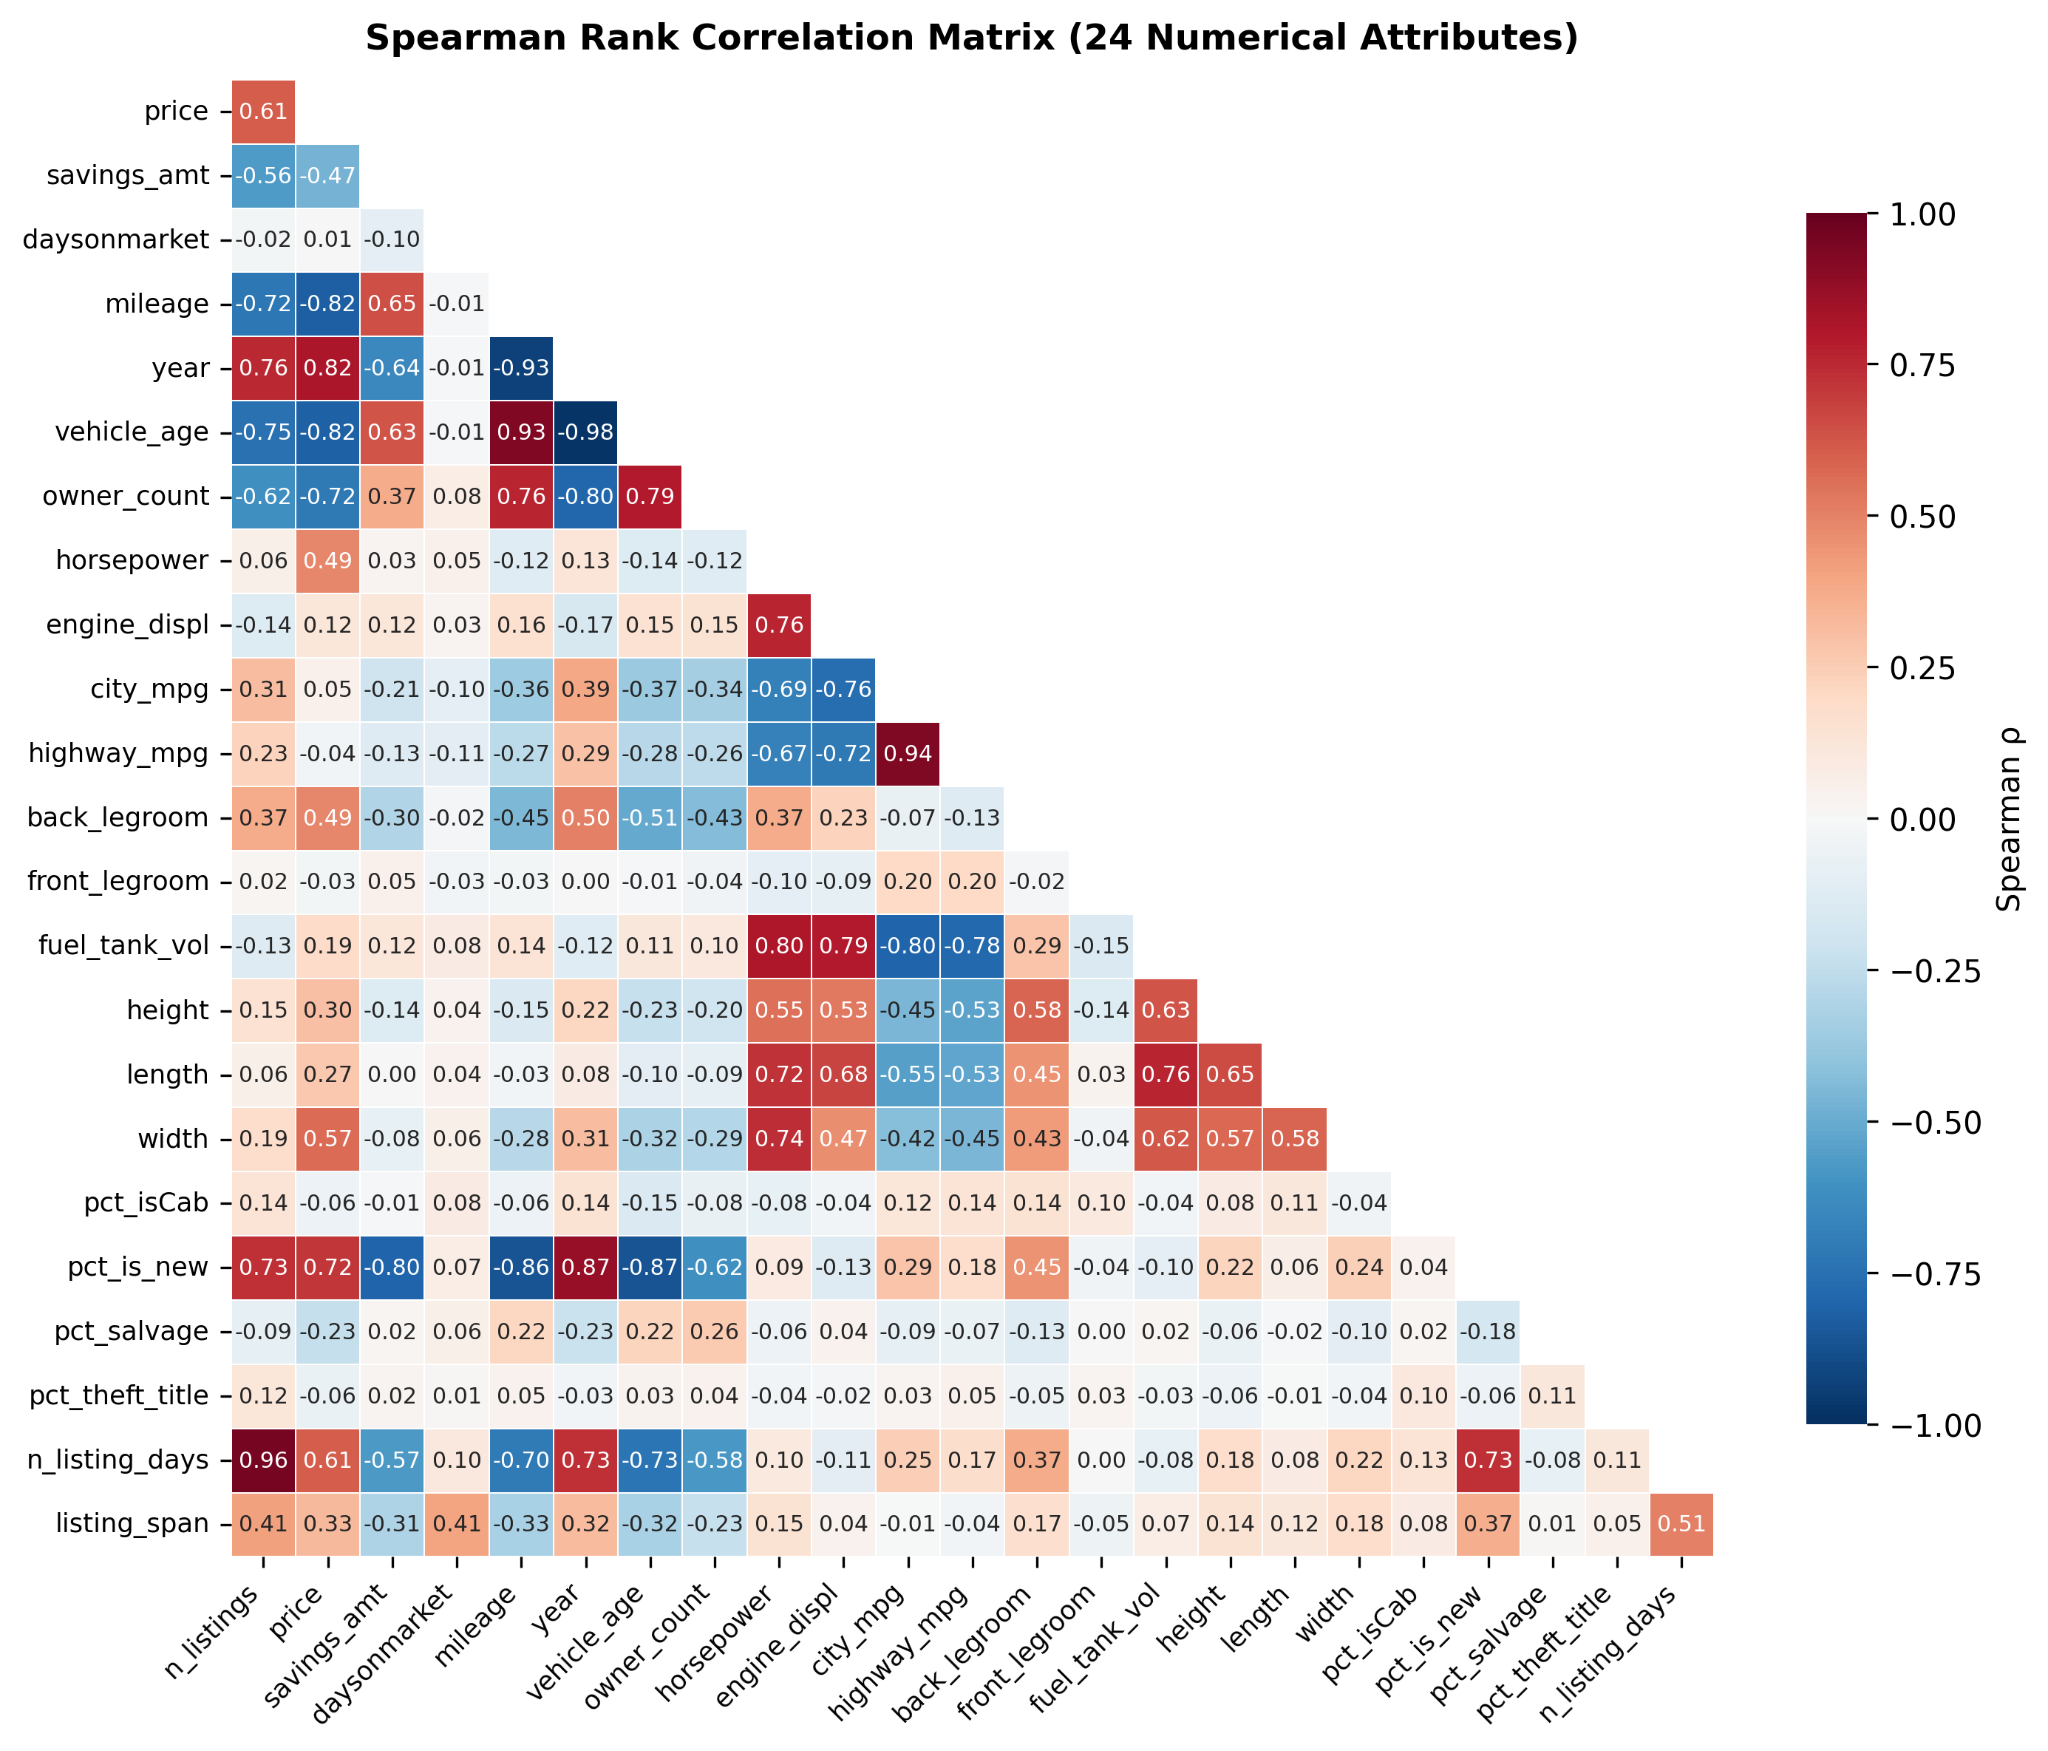
\includegraphics[width=\linewidth]{figures/docx/fig_1_7_correlation.png}
  \captionof{figure}{Spearman correlation matrix of the numerical attributes.}
  \label{fig:corr}
\end{minipage}
\end{figure}

\FloatBarrier

%=====================================================================
\section{Clustering}
\label{sec:clustering}
\emph{(TODO: describe the clustering setup, the features used, and how
dimensionality reduction was applied.)}

\subsection{Centroid-based}
\emph{(TODO: K-Means; elbow and silhouette for choosing $K$.)}

\subsection{Density-based}
\emph{(TODO: DBSCAN; $k$-NN distance plot to choose $\varepsilon$ and MinPts.)}

\subsection{Hierarchical}
\emph{(TODO: agglomerative clustering; linkage comparison and dendrograms.)}

\subsection{Final discussion}
\emph{(TODO: compare the methods and state which worked best.)}

%=====================================================================
\section{Classification}
\label{sec:classification}
The target variable is \texttt{seller\_rating\_class}. Describe the
preprocessing, the train/test split, and the evaluation metrics (accuracy,
precision, recall, F1, ROC-AUC).

\subsection{KNN}
\emph{(TODO: hyperparameter search results and per-class metrics.)}

\subsection{Na\"ive Bayes}
\emph{(TODO: Gaussian and/or Categorical Naive Bayes results.)}

\subsection{Decision Trees}
\emph{(TODO: tuning, pruning, and the resulting tree.)}

\subsection{Final conclusion}
\emph{(TODO: compare all classifiers and recommend one.)}

\begin{table}[h]
  \centering
  \caption{Model comparison. \emph{(Fill in.)}}
  \label{tab:clf-results}
  \footnotesize
  \setlength{\tabcolsep}{3pt}
  \begin{tabular}{lccc}
    \toprule
    Model & Accuracy & Macro-F1 & Macro-AUC \\
    \midrule
    k-NN & & & \\
    Na\"ive Bayes & & & \\
    Decision Tree & & & \\
    \bottomrule
  \end{tabular}
\end{table}

%=====================================================================
\section{Regression}
\label{sec:regression}
\emph{(TODO: describe the regression target and predictors.)}

\subsection{Univariate regression}
\emph{(TODO: simple regression per predictor.)}

\subsection{Multivariate regression}
\emph{(TODO: multiple and multi-target regression.)}

%=====================================================================
\section{Pattern Mining}
\label{sec:patterns}
\emph{(TODO: describe the discretization/binning of numeric attributes and the
transactional representation.)}

\subsection{Frequent patterns}
\emph{(TODO: Apriori vs FP-Growth, support and itemset-size analysis.)}

\subsection{Association rules}
\emph{(TODO: top rules, support/confidence/lift, and interpretation.)}

%=====================================================================
\section{Conclusion}
\label{sec:conclusion}
\emph{(TODO: summarise the findings and the main takeaways.)}

\section*{Team Contributions}
\label{sec:contributions}
\begin{table}[h]
  \centering
  \small
  \begin{tabularx}{\columnwidth}{l X}
    \toprule
    Member & Contribution \\
    \midrule
    \memberA & \\
    \memberB & \\
    \memberC & \\
    \bottomrule
  \end{tabularx}
\end{table}

\end{document}
